\pgfplotstablegetelem{\thepart}{[index]\columnIndex}\of{\cronograma}
\part{\pgfplotsretval}
\label{part:\thepart}
\frame{\partpage}

\begin{frame}[t]{Soft Skills}
	
	\vspace{1em}
	
	\fontsize{16pt}{15}\selectfont{
		São habilidades subjetivas.
	}\par
	\vspace{1em}
	
	\fontsize{16pt}{20}\selectfont{
		\begin{itemize}%[<+->] 
			
			\item Tem muita relação com a inteligência emocional.
			\item Muitas vezes são difíceis de serem identificadas e definidas.
			
		\end{itemize}
	}\par
	\vspace{1em}
	
\end{frame}


\begin{frame}[t]{Soft Skills}
	\vspace{1em}

	\fontsize{16pt}{20}\selectfont{
		\begin{itemize}%[<+->] 
			
			\item Para entender a importância das soft skills é preciso deixar claro a sua definição.
			
			\item Porém não é fácil definir soft skills, pois essa definição pode variar com o contexto, por exemplo: uma competência que pode ser considerada soft skills numa área e pode ser considerada hard skill em outras áreas.
			
		\end{itemize}
	}\par
	\vspace{1em}

\end{frame}



\begin{frame}[t]{Soft Skills}
	Algumas boas definições.
	\vspace{1em}
	
	\fontsize{14.5pt}{20}\selectfont{
		\begin{itemize}%[<+->] 
			
			\item Competências comportamentais referentes a traços de personalidade e atitudes que guiam o comportamento do indivíduo.
			
			\item Combinação de qualidades pessoais, habilidades interpessoais, habilidades e conhecimentos adicionais que ajudam a obter uma boa performance profissional.
			
			\item Conjunto de competências e habilidades pessoais que descrevem as interações sociais,
			principalmente no ambiente de trabalho, além disso ditam a atitude de cada um e sua a
			compatibilidade com os outros.
			
		\end{itemize}
	}\par
	\vspace{1em}
	
\end{frame}



\begin{frame}[t]{Soft Skills}

	\fontsize{12pt}{15}\selectfont{
		Soft skills encontradas no Computing Curricula de 2020 (p.50). \href{https://www.acm.org/binaries/content/assets/education/curricula-recommendations/cc2020.pdf}{Veja aqui}.
	}\par
	\vspace{0.5em}
	
	\fontsize{12pt}{15}\selectfont{
		\begin{itemize}%[<+->] 
			
			\item Pensamento Analítico e Crítico.
			\item Colaboração e Trabalho em Equipe.
			\item Perspectivas Éticas e Interculturais.
			\item Priorização e gerenciamento de multitarefas.
			\item Comunicação Oral e Apresentação.
			\item Resolução de problemas.
			\item Proatividade.
			\item Comunicação escrita.
			\item Gerenciamento de tempo.
			\item Autodidatismo.
			
		\end{itemize}
	}\par
	\vspace{1em}
	
\end{frame}




\begin{frame}[t]{Soft Skills}

	\fontsize{14pt}{18}\selectfont{
		\begin{itemize}%[<+->] 

			\item Boas habilidades sociais têm um impacto positivo no ambiente de trabalho e na carreira dos profissionais.

			\item Entre as soft skills importantes, destacam-se a comunicação e a criatividade.

			\item A proficiência na comunicação oral e escrita é considerada um requisito mínimo para alguns cargos e carreiras.

			\item Além disso, a criatividade, muitas vezes vista como uma habilidade exclusiva de artistas, é essencial para encontrar soluções inovadoras para problemas.

		\end{itemize}
	}\par
	\vspace{1em}

\end{frame}





\begin{frame}[t]{Soft Skills}
	
	\fontsize{16pt}{20}\selectfont{
		\begin{itemize}%[<+->] 
			
			\item Para ter sucesso no mercado de trabalho, os candidatos a emprego precisam ter uma
			vantagem competitiva sobre os outros candidatos com qualificações técnicas semelhantes, é aí
			que as soft skills se encaixam.
			
			\item Os empregadores preferem candidatos que estejam prontos para trabalhar, se uma pessoa (potencial empregado) tiver que ser treinado, em relação a soft skills, antes de se tornar produtivo para empresa, isso lhe dará uma desvantagem competitiva.
			
		\end{itemize}
	}\par
	\vspace{1em}
	
\end{frame}





\begin{frame}[t]{Soft Skills}

	\fontsize{16pt}{20}\selectfont{
		\begin{itemize}%[<+->] 

		\item Durante a entrevista de emprego boas habilidades de comunicação são muito importantes e podem camuflar a falta de habilidades técnicas.
		
		\item Boas habilidades técnicas não são necessariamente suficientes para que um funcionário receba uma
		promoção, os empregadores preferem promover funcionários com soft skills bem desenvolvidas.

		\end{itemize}
	}\par
	\vspace{1em}

\end{frame}

\begin{frame}[t]{Soft Skills}

	\vspace{1em}
	\centering
	Avaliação de empregadores de quais soft skills são essenciais para ter uma carreira bem sucedida
	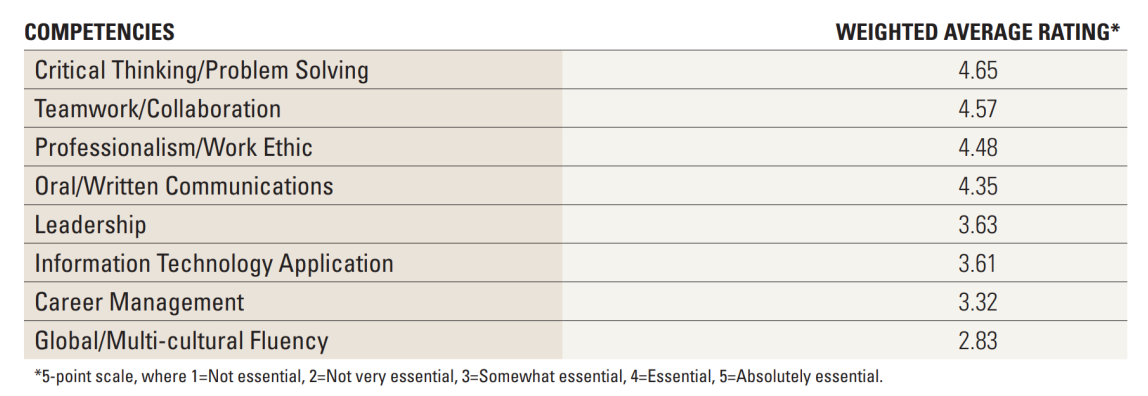
\includegraphics[width=0.9\textwidth]{imagens/fig-soft-skills-pesquisa.png}\\
	Fonte: Job Outlook 2020 Survey \href{https://in.nau.edu/wp-content/uploads/sites/204/2020-nace-job-outlook.pdf}{Leia mais aqui}
	
\end{frame}




